\documentclass{report}
\pagestyle{plain}
\pagenumbering{arabic}

\usepackage[utf8]{inputenc}
\usepackage[T1]{fontenc}
\usepackage{textcomp}

\usepackage{amsmath}
\usepackage{amsfonts}
\usepackage{amssymb}
\usepackage{array}
\usepackage{amscd,amsmath,amssymb,amstext,amsthm}
\usepackage{braket}
\usepackage{enumitem}
\usepackage{mathpartir}
\usepackage{tikz}
\usepackage[utf8]{inputenc}
\usepackage[T1]{fontenc}
\usepackage{textcomp}
\usepackage{ulem}
\usepackage{booktabs}
\usepackage{setspace}
\usepackage{longtable}
\usepackage{sectsty}
\usepackage{titlesec}
\usepackage{titling}
\usepackage[numbers]{natbib}
\usepackage{graphicx}
\usepackage{caption}
\usepackage{threeparttable}
\usepackage{threeparttablex}
\usepackage{placeins}
\usepackage{subcaption}
\usepackage{textgreek}
\usepackage[version=3]{mhchem}
\usepackage[nottoc]{tocbibind}
\usepackage{xcolor}
\usepackage{listings}
\usepackage{tikz}
\usetikzlibrary{shapes,arrows,positioning} 
\usetikzlibrary{calc}
\usetikzlibrary{arrows.meta}
\usetikzlibrary{positioning}

\definecolor{codegreen}{rgb}{0,0.6,0}
\definecolor{codegray}{rgb}{0.5,0.5,0.5}
\definecolor{codepurple}{rgb}{0.58,0,0.82}
\definecolor{backcolour}{rgb}{0.95,0.95,0.92}

\lstdefinestyle{mystyle}{
    backgroundcolor=\color{backcolour},   
    commentstyle=\color{codegreen},
    keywordstyle=\color{magenta},
    numberstyle=\tiny\color{codegray},
    stringstyle=\color{codepurple},
    basicstyle=\ttfamily\footnotesize,
    breakatwhitespace=false,         
    breaklines=true,                 
    captionpos=b,                    
    keepspaces=true,                 
    numbers=left,                    
    numbersep=5pt,                  
    showspaces=false,                
    showstringspaces=false,
    showtabs=false,                  
    tabsize=2
}
\lstset{style=mystyle}

\DeclareUnicodeCharacter{2009}{ }

\definecolor{darkblue}{rgb}{0,0,0.7}
\usepackage{hyperref}
\usepackage{url}
%\usepackage{breakurl}
\def\UrlBreaks{\do\/\do-}


\usepackage
[
        a4paper,
        left=30mm,
        right=25mm,
        top=25mm,
        bottom=25mm,    
]
{geometry}

\makeatletter
    \renewcommand{\@makechapterhead}[1]{%
    \vspace*{50 pt}%
    {\setlength{\parindent}{0pt} \raggedright \normalfont
    \bfseries\Huge\sffamily
    \ifnum \value{secnumdepth}>1 
        \if@mainmatter\thechapter.\ \fi%
    \fi
    #1\par\nobreak\vspace{40 pt}}}
    \makeatother

\newcommand{\subtitle}[1]{%
  \posttitle{%
    \par\end{center}
    \begin{center}\large#1\end{center}
    \vskip4em}%
}	

\newcommand*\PrintSkips[1]{%
  \typeout{In #1:}%
  \typeout{\@spaces above: \the\abovecaptionskip}%
  \typeout{\@spaces below: \the\belowcaptionskip}%
}

\newcommand{\tu}{\textmu}

\NewDocumentCommand{\codeword}{v}{%
\texttt{\textcolor{black}{#1}}%
}

\newcolumntype{P}[1]{>{\raggedright\arraybackslash}p{#1}}  

\begin{document}
\allsectionsfont{\sffamily}
\onehalfspacing

\setlength\parindent{0pt}
  

\title{\sffamily Developing an R package for quantitative analyses of T cell/tumour cell contacts \vskip4em}
\subtitle{\sffamily
 \large \textbf{Masterarbeit\\ and der Medizinischen Fakultät \\der Eberhard Karls Universität Tübingen}}
\author{\large \sffamily vorgelegt von \vspace{2ex}\\ \sffamily \textbf{Quach, Julia}}
\date{\large \sffamily\textbf{Tübingen, DATUM}}
\maketitle

\chapter*{Statement}

I hereby declare:
\begin{itemize}
\item that this thesis is my own work and that I have not made use of any other sources or aids than those referenced.
\item that all statements appropriated from other works in letter or in substance have been referenced as such. 
\item that the thesis submitted has not been the subject of any other examination in essential parts or in full
\item that the thesis submitted has not been published in essential parts or in full.
\end{itemize}


\noindent I affirm that I have written the dissertation myself and have not used any sources and
aids other than those indicated.
The references are presented accorded to standard rules for publication and
standard citation guidelines.\\\\


\noindent Tübingen, Date, Signature


\tableofcontents
%===================================================

\setlength\parindent{0pt}

\chapter{Summary}

To do:
\begin{itemize}
	\item Edit description of R package
	\item Add results and discussion part to summary
\end{itemize}

With nearly 10 million deaths in 2020, cancer is one of the leading causes of death worldwide \citep{WHO}\citep{WHO_Cancer}. Its high mortality is predominantly caused by resistance against available cancer therapies [c]. To combat this resistance, new therapies have been developed from which immunotherapeutic approaches have demonstrated promising results [c]. Those immunotherapies make use of engineered or innate immune cells, especially T cells, to eliminate malignancies [c]. Nevertheless, solid cancer types often remain resistant due to their immunosuppressive tumour microenvironment [c]. To overcome this hurdle, it is essential to understand the crucial factors promoting successful T cell killing. 

To deepen our understanding of T cell killing, a very intuitive method is to \textit{watch} the T cells while interacting with tumour cells by using live-cell imaging methods combined with a range of labelling techniques. For this, the OVA (ovalbumin)-tumour model comes handy as it provides tumour cell lines expressing the OVA antigen and transgenic mice expressing OVA-targeting T cells. 

The interaction between T cells and tumour cells is essential for T cell killing. To quantitatively analyse this cell-cell interaction, we developed a work flow which includes the segmentation and tracking of tumour and T cells and the detection of cell-cell contacts. For the latter, we built an R package \textit{cellcontacts} to identify cell-cell contacts and compute their frequency and duration. Furthermore, the R package is capable of mapping the interaction analyses to immunological staining results.

To put it in a nutshell, this thesis' aim is to widen the explanatory power of available live-cell imaging techniques by enabling large-scale analyses of cell interaction and correlation to immunological staining methods. We show that [...]

%%===================================================
\chapter{Introduction}

%\begin{itemize}
%	\item Why T cells are crucial for tumour elimination
%	\item Crucial factors for T cell killing and the relevance of cell dynamics
%	\item Tools to investigate cell dynamics
%	\item Software to analyze cell tracks
%\end{itemize}

In this section, we will introduce the essential role of T cells for tumour cell elimination and afterwards, we will focus on the crucial factors for efficient T cell killing. We will explain the necessity to understand cell dynamics for unravelling T cell killing mechanisms. Eventually, we will address available tools to analyse cell movement.

\section{T cells are crucial for tumour elimination}

To do:
\begin{itemize}
	\item Mention anti-tumour activity of NK cells
	\item Compare NK cells vs. T cells
\end{itemize}

Cancer is a disease in which body cells grow uncontrollably because of inherited or acquired mutations [c]. Those cells form tissue mass, called malignant tumours, that can spread over the body, impede normal body cells and cause disease [c].
Naturally, the immune system is capable to track down and eliminate such abnormal cells by inducing their cell death. For this, T cells, a type of immune cell, use their surface antigen receptors to find irregularities within the surface antigens of abnormal cells. If they find suspicious cells, T cells induce their apoptosis, a well-regulated cell death.
In accordance, malfunction of the immune system is strongly correlated to a higher incidence of cancer [ccc]\citep{RN295}. In particular, a decline in T cell mediated immune response can lead to a reduced response against malignant tumour cells and cause disease \citep{RN295}.
In conclusion, if the mechanisms to eliminate abnormal cells are suppressed or fail, cancer cells can form malignant tumours. To prevent the formation of malignant tumours, T cells play a key role as they are capable of eliminating tumour cells.

\section{CAR T cell therapy exploits the killing activity of T cells}

To-do:
\begin{itemize}
	\item Add some statistics and citations on antibody and CAR T cell therapy
\end{itemize}

Because T cells are capable of eliminating tumour cells, it is clear that one would like to enhance their killing activity to prevent and treat cancer. To achieve this goal, we need to understand why natural T cells are not always capable of full tumour elimination: Researchers found that tumour cells can escape immuno-surveillance through inhibiting T cell activity, down-regulating their surface antigens, and inducing T cell exhaustion [ccc]. 

Understanding these immune escape mechanisms, allowed two major breakthroughs in cancer therapy: 
Check-point inhibitors were discovered which can reverse an inhibition on T cell activity. The release of this brake allows T cells to become active and track down and kill cancer cells [ccc]. This finding was awarded with a Nobel Prize in 2018 and the consequent therapeutic approaches, called antibody therapies, became a standard in the clinics [c]. 

Even with a released brake, T cells are not able to track down tumour cells that hide by down-regulating their surface-antigens. To tackle this obstacle, researchers have genetically engineered T cells that  carry modified antigen receptors such that they can identify and kill hiding tumour cells [c]. This approach, called chimeric antigen receptor (CAR) T cell therapy, was successful in treating leukaemia cases that were incurable before [cc]. Hence, it was a second major breakthrough in cancer therapy [cc]. 

Following the great success of CAR T cell therapy to treat haematological malignancies, efforts have sparked to translate this approach to solid tumour entities [ccc]. But in contrary to leukaemia, solid tumours have a often times stiff tumour micro-environment which consists of an extracellular matrix filled different non-cancerous cell types [ccc]. This makes it difficult for T cells and CAR T cells to even enter the tumour tissue before they have a chance to identify and kill the tumour cells [ccc]. Once T cells got through the tumour micro-environment and arrived at the tumour cells, they are usually exhausted and their killing activity is drastically reduced [cc]. 

To increase the success of CAR T cell therapy in solid malignancies, one could either tackle the tumour micro-environment or further modify CAR T cells such that they become more effective even in an exhaustive environment. There is much research approaching both ideas and adequate methods are required to evaluate the success of those modifications [cc]. In the following section, we will put our focus on the methods to evaluate the success of tumour treatments. Furthermore, we will address why the investigation of cell dynamics is pivotal to evaluate the success of T cell killing.


\section{Why are cell dynamics relevant?}

\begin{itemize}
	\item Describe tools to evaluate CAR T cell efficiency
	\item Name the advantages and also shortcomings of static methods (FACS, sequencing, immuno-stainings)
	\item Name the benefit of cell dynamics
	\item In particular:
		\begin{itemize}
	\item Explain why understanding cell-cell interactions are essential for tumour killing
	\item What is known about cell-cell interaction and what we would like to know about cell-cell interaction
\end{itemize}

\end{itemize}

To observe the success of T cell killing, the most straightforward approach would be to measure the amount of surviving tumour cells before and after therapy. But this is neither sufficient nor does this method reveal the full picture: It does not give an insight into [name more reasons]\\


Hence, the interaction between T cells, tumour cells and their tumour micro-environment should be observed from different angles which we can roughly classify into static and dynamic methods: Static methods give a detailed insight into the cellular processes at a specific point, including the gene and protein expression profile of cells on a single cell-level, the distribution of cells in tissue and the cells' state in the cell cycle [ccc]. 
%Examples for static methods include flow cytometry, DNA- and RNA-sequencing techniques and immunological staining of tissue and cell samples. 
On the other hand, dynamical methods are able to capture immune and tumour cells on a temporal scale. They widen our understanding of cell-cell-interaction, cell growth and killing activity [ccc]. For example, \textit{in vitro} live-cell imaging can visualize how tumour cells move during tumour growth and invasion and with additional labelling of $\text{Ca}^{2+}$-signalling, we can investigate \textit{when and how} the T cells try to kill tumour cells. [Mention additive cytotoxiciy and maybe also other papers] \\


Given the different aspects that static and dynamic methods elucidate, it is beneficial to join forces to understand and modify existing tumour therapies. For this, we need comprehensive analysis work flows that combine results from static and dynamic experiments.

In the following section, we will give an overview of existing tools to investigate cell dynamics in live-cell imaging films. In the end, we will give an insight into available tools to combine static with dynamic methods to understand T cell killing mechanisms.

\section{Tools to investigate cell dynamics}

Cell dynamics are equally important as static cell information. In this project, we will first put our focus on methods to quantitatively analyse cell dynamics and cell-cell interaction. Following, we will address methods to connect results on cell dynamics to the findings from static experiments.

Live-cell imaging techniques usually produce a file of around 35 GB file size with around 3000 frames capturing a region of interest of around $\color{cyan}{x} \times \color{cyan}{x}$ \textmu m with around \textcolor{cyan}{x} cells for \textcolor{cyan}{x} hours. After acquiring such a data set, it is evident that it is not feasible to analyse the whole data set manually. Therefore, tools which can automatically detect cells and track their movement are indispensable. In this section, we will introduce available tools for automated cell segmentation and tracking.

\subsection{Cell segmentation}

\begin{itemize}
	\item Stardist
	\item CellPose
\end{itemize}

Before analysing cell movement, cells need to be automatically identified and their boundary accurately delineated, called segmented. For this purpose, several cell segmentation tools have been published [ccc]. Within these tools, StarDist has proved to be reliable for an automatic detection of cell nuclei in a regular roundish shape. The core of StarDist is a convolutional network which has been trained to predict the occurrence of a polygon representing the cell nucleus shape for every pixel. This approach facilitates the correct segmentation of crowded cells which is a typical phenomenon in live-cell imaging although it does not allow the segmentation of ring- or in general odd-shaped cell nuclei \citep{RN285}. 
%Another cell-segmentation tool is CellPose

\subsection{Cell tracking}

\begin{itemize}
	\item Overview and classification
	\item LAP tracker
	\item Kalman tracker
\end{itemize}

Regarding the tracking of cell movement, there exist a broad range of algorithms [cc]. A comprehensive analysis of available cell-tracking algorithms was given by Ulman \textit{et al} in which 21 cell-tracking algorithms were classified regarding their tracking strategy and evaluated based on their performance on up to 13 data sets.
In terms of the tracking strategy, the algorithms either used cell contour evolution techniques or cell detection methods. The former requires a spatio-temporal overlap between the corresponding cell regions, thus performing segmentation and tracking in one task, whereas the latter firstly segments the cells in all frames and afterwards, builds a probabilistic framework to propose temporal associations between the cells. While some tracking algorithms achieved good results, none of them achieved fully correct solutions for all data sets. Hence, a major implication of this report is that the right choice of tracking algorithm heavily depends on the applied imaging modality and the respective data set \citep{RN292}. 

[More information on T cell tracking, segmentation + detection and not cell contour evolution]

To facilitate the usage of cell-tracking algorithms, the extensible, open-source Fiji plugin \textit{TrackMate} was published by Tinevez \textit{et al} \citep{RN293}. Via a graphical user interface, it allows the user to choose a segmentation algorithm and a tracking algorithm for their specific data set in any combination. The available segmentation algorithms included ilastik, Weka, cellpose, MorphoLibJ and StarDist. Moreover, TrackMate allows the import of segmentation results as mask or label images. For the tracking algorithm, TrackMate offers the LAP framework by Jaqaman \textit{et al} for Brownian motion [c] and the Kalman filter for linear motion [c]. Overall, TrackMate offers an open-source framework to combine any segmentation and tracking algorithm for a customized cell-tracking work flow.


\subsection{Cell-cell contacts}

\begin{itemize}
	\item Available tools
	\item Our needs -> quantitative information from microscopy images of cultured cells
\end{itemize}

To gain biological insights from time-lapse microscopy recordings of cell behaviour, ...


How do the dynamics of T cell behaviour correlate to tumour killing efficiency? This is the question central to this thesis. 


%===================================================
\chapter{Data sets}
%===================================================

We used five live-cell imaging datasets to build and to challenge the R package. All data sets were acquired using a Widefield Microscope DMI8 by Leica Microsystems (Wetzlar, GER) as imaging device equipped with a \textcolor{blue}{[...]} objective with a resolution of \textcolor{blue}{[...]} at 5\% $\text{CO}_2$.

To set the distance and duration thresholds for cell-cell contact computation, we used three data sets of live-cell imaging films with tumour and T cells. An overview of the data sets is given in Table \ref{Datasets_building}.

% Table of training data sets
\begin{table}[h!]
\centering
\caption[Data sets to build the work flow]{Overview of data sets that were used for building the R package} \label{Datasets_building}

\begin{tabular}{ P{2.5cm} P{2.5cm}  P{2cm} P{2cm} P{2cm} P{2cm}} 
Tumour cell line 	& T cell line	& Frame rate & Frame size &  Duration & Temperature\\
					& 				& (sec/frame)&(\tu m $\times$ \tu m) & (h) & $(^\circ \text{C})$\\ \midrule
\textcolor{blue}{YUMM-OVA (add cell concentration)} &  				&  &   &  &  \\[10pt]
\textcolor{blue}{YUMM} &  				&  &   &  &  \\[10pt]
\textcolor{blue}{Ovarian} &  				&  &   &  &  \\[10pt]
\end{tabular}
\end{table}

To challenge the work flow for cell-cell contact detection, we applied the image analysis pipeline on three additional data sets (see Table \ref{Datasets_challenging}).

% Table of challenge data sets
\begin{table}[h!]
\centering
\caption[Data sets to challenge the work flow]{Overview of data sets that were used for challenging the R package} \label{Datasets_challenging}

\begin{tabular}{ P{2.5cm} P{2.5cm}  P{2cm} P{2cm} P{2cm} P{2cm}} 
Tumour cell line 	& T cell line	& Frame rate & Frame size &  Duration & Temperature\\
					& 				& (sec/frame)&(\tu m $\times$ \tu m) & (h) & $(^\circ \text{C})$\\ \midrule
\textcolor{blue}{YUMM} &  				&  &   &  &  \\[10pt]
\textcolor{blue}{YUMM-OVA} &  				&  &   &  &  \\[10pt]
\textcolor{blue}{B16F10} &  				&  &   &  &  \\[10pt]
\end{tabular}

\end{table}

%===================================================
\chapter{Method}
%===================================================

The R package \textit{cellcontacts} was built to process cell tracks acquired from live-cell imaging films of tumour cells with T cells. The package is meant to detect and characterise cell-cell contacts and cell movement for large data sets. Moreover, it relates cell-cell contacts and cell movement to findings from immunological staining techniques. The package requires preprocessing of live-cell imaging films with a cell tracking tool, e.g., \href{https://imagej.net/plugins/trackmate/}{TrackMate} or \href{https://imaris.oxinst.com/products/imaris-for-tracking}{Imaris}. 
In this chapter, the package's algorithm to compute cell-cell contacts is described and an analysis pipeline incorporating TrackMate and the R package \textit{cellcontacts} is laid out.

\section{Algorithm to compute cell-cell contacts}

In this section, we formally define cell-cell contacts. Afterwards, we describe the algorithm to compute cell-cell contacts.

\paragraph{Formalizing the data set and defining cell-cell contacts} 
Let $n \in \mathbb{N}$ be the the last time point in the live-cell imaging film, equivalent to the maximum frame number. 
Let $M_i$ be the set of all cells at one time point $i \in \{1, \dots, n\}$ with $0 \in M_i$ representing a non-registered cell. Let $U_i \subset M_i$ be the set of tumour cells and $V_i \subset M_i$ the set of T cells at a time point $i \in \{1, \dots, n\}$ such that $M_i = U_i \cup V_i$. \\

A tumour cell shall be represented as $u = (u_1, \dots, u_n) \in U_1 \times \dots \times U_n$ such that for each time point $i \in \{1, \dots, n\}$, the element $u_i$  either represents the xy-position of the tumour cell at this time point or equals $0$ if the respective tumour cell was not registered at this time point. Analogously, we define T cells as $v = (v_1, \dots, v_n) \in V_1 \times \dots \times V_n$.\\

Let $d_i: U_i \times V_i \to \mathbb{R}$ be a metric that describes the euclidean distances between the segmented area of tumour cell and a T cell for a given time point $i \in \{1, \dots,n\}$ and if either the tumour cell or the T cell was not registered during that time point, we define $d_i(u_i, v_i) = \infty$.\\

Let $x \in \mathbb{R}$ be a distance threshold in \textmu m and $m \in \mathbb{N}$ a duration threshold given as number of frames. We define that a tumour cell $u \in U_1 \times \dots \times U_n$ and a T cell $v \in V_1 \times \dots \times V_n$ are \textit{in contact} if and only if their distance is below the distance threshold for $m$ consecutive frames:
\begin{equation*}
	u \text{ and } v \text{ in contact } 
		\quad \Leftrightarrow \quad 
		\exists \, j \in \{1, \dots, n\} \;
		\forall i \in \{j, \dots, j+m\}: \;
	 	d_i(u_i, v_i) \le x
\end{equation*}

\paragraph{Algorithm (cell-cell contact computation)} To compute cell-cell contacts, we need to find all tumour cell/T cell pairs $(u,v)$ that maintain a distance below threshold for $m$ consecutive frames. As the number of distance calculations grow quadratically with an increasing frame size of the film, we added preprocessing steps to fasten the computation time:\\


\begin{center}
\fbox{
\parbox{\textwidth}{
\smallskip

\begin{center}
\textbf{Algorithm to compute cell-cell contacts}
\end{center}
\textbf{Input}: 
	\begin{itemize}
		\item Cell tracks and cell areas of tumour cells and T cells at all time points.
		\item A distance threshold $x$.
		\item A minimum duration threshold expressed as a number of frames $m$.
	\end{itemize}
\textbf{Output}: Data frame with columns  
	\begin{itemize}
		\item Names of cell pairs that maintain a distance below threshold for at least $m$ consecutive frames.
		\item Time points during a contact.			
		\item Cell-cell distances during a contact.
	\end{itemize}
\textbf{Instructions}: 
\begin{enumerate}
	\item Preprocessing
		\begin{enumerate}[label=1.\arabic*]
			\item Compute the center points of all tumour and T cells.
			\item Create a grid in which columns and rows have a distance of 100\,\textmu m.
			\item Sort the computed cell center points into the grid.
		\end{enumerate}
	\item Distance computation
		\begin{enumerate}[label=2.\arabic*]
			\item Compute all possible tumour cell/T cell pairs for each time point.
			\item For each pair, save the information whether their grid coordinates are farther away than two rows or columns. 
			\item If the grid coordinates are at least in neighbouring rows and columns, compute and save the distance of the segmented tumour and T cell area.
		\end{enumerate}
	\item Filtering for contacts 
		\begin{enumerate}[label=3.\arabic*]
			\item For all time points, discard cell pairs that have a distance above the threshold $x$.
			\item For the remaining pairs, discard cell pairs that maintain a distance below threshold for less than $m$ frames.	
			\item Return the pair names, their distance and their time point information as a data frame.
		\end{enumerate} 
\end{enumerate}
}
}
\end{center}


\section{Proposed image analysis pipeline}

After describing the algorithm, this section is a detailed guide through the image analysis work flow. An overview of the steps in the work flow is given in Figure \ref{Workflow_overview}. An exemplary R script is provided on the \href{https://github.com/juliaquach02/cellcontacts}{GitHub page} of the R package and a detailed tutorial of the workflow is provided in the supplement (\textcolor{blue}{add link}).
% Overview
\begin{figure}
\caption[Workflow_Overview]{Overview of work flow to detect cell-cell contacts in live-cell imaging films using the R package \textit{cellcontacts}. \label{Workflow_overview}}
\centering
\tikzstyle{block} = [rectangle, draw,
    text width = 15cm, text centered, rounded corners, inner ysep=10pt]
\tikzstyle{line} = [draw, -latex']

\begin{tikzpicture}[node distance = 1cm, auto]
    \node(Setup) [block]  { 
    		\textbf{Setup} \begin{itemize}
    		\item Installation of ImageJ with StarDist and TrackMate plugin.
    		\item Installation of RStudio with \textit{cellcontacts} package and dependencies.
    	\end{itemize}
    };
    \node(Preprocessing) [block, below =of Setup] {
    		\textbf{Preprocessing in ImageJ} \begin{enumerate}
			\item Loading of the live-cell imaging film as .tif file with at least two channels for tumour and T cells. Both cell types need to be fluorescent.    		
    		\item Segmentation and tracking of tumour cells and T cells in the TrackMate plugin.
			\item Export of cell ROIs as .roi files in zipped folders and cell tracks as .csv file with columns for the cell ID, time point and the xy-coordinates.
    \end{enumerate}
    };
    \node(Computation) [block, below =of Preprocessing] {
    		\textbf{Analysis in RStudio} \begin{enumerate}
    		\item Setting source and destination directories and loading of \textit{cellcontacts} library. 
			\item Importing cell tracks as data frame as .csv file and cell ROIs from zipped folders with .roi files.
			\item Matching the track names to their respective frame number.
			\item Rearranging data set into hash maps.
			\item Computing cell-cell distances.
			\item Filtering for cell-cell contacts.
			\item Exporting the data frame with cell-cell contacts as .csv file.
    \end{enumerate}
    };
    \node(Validation) [block, below =of Computation] {
    		\textbf{Validation in ImageJ} \begin{enumerate}
    		\item Import of the computed cell-cell contacts via the TrackMate CSV importer.
    		\item Checking the live-cell imaging film with the labelled tumour cell/T cell contacts.
    \end{enumerate}
    };
    \node(Further analysis) [block, below =of Validation] {
    		\textbf{Statistcal analyses in RStudio} \begin{enumerate}
    		\item Connecting the computed cell-cell contacts to results from immunological staining.
    		\item Performing statistical analysis on the results.
    \end{enumerate}
    };
    % Draw edges
    \path [line] (Setup) -- (Preprocessing);
    \path [line] (Preprocessing) -- (Computation);
    \path [line] (Computation) -- (Validation);
	\path [line] (Validation) -- (Further analysis);
    
\end{tikzpicture}
\end{figure}

\paragraph{Requirements}
To use this work flow on a live-cell imaging film, the imaged cells need to be fluorescent to enable their correct segmentation. The frame rate usually needs to be 90\,s/frame or faster to ensure correct tracking of fast-moving T cells.

To process the live-cell imaging films, installation of the open source package \href{https://imagej.net/software/fiji/}{Fiji} (also known as ImageJ) with the plugins \href{https://imagej.net/plugins/stardist}{StarDist} for cell segmentation and \href{https://imagej.net/plugins/trackmate/}{TrackMate} for cell tracking is required.
To use the \textit{cellcontacts} package, the programming language \href{https://cran.r-project.org/bin/windows/base/}{R} is needed, preferably in the \href{https://posit.co/download/rstudio-desktop/}{RStudio environment}.

\paragraph{Installation}
The latest development version of \textit{cellcontacts} can be installed in the R environment after getting access to the \textit{cellcontacts} project on GitHub:
\begin{lstlisting}[language=R]
	devtools::install_github( "juliaquach02/cellcontacts" ) 
\end{lstlisting}
The package can be loaded via:
\begin{lstlisting}[language=R]
	library( cellcontacts )
\end{lstlisting}

\paragraph{Preprocessing in ImageJ} 
To extract the image features, we load the live-cell imaging film as .tif-file into Fiji where we can use the TrackMate plugin for segmentation and tracking. Two separate TrackMate session are needed to analyse T cells and tumour cells. During segmentation and tracking, the plugin offers the possibility to adjust parameters and to manually correct segmented cells or cell tracks if necessary. After segmentation and tracking, the cell areas of both data sets are renamed in the TrackMate GUI by their assigned track name and an unique index for the respective track. 

We export cell tracks as .csv file with columns indicating the cell ID, time and coordinates at each measured time point.
%By default, the first three lines of the .csv file contain the header of its columns in three different text styles (capital letters, full name and abbreviated). To enable correct loading of the .csv files with R, two of the first three lines are deleted, e.g. via a text editor.
The renamed cells region of interests (ROIs) are exported as several zipped folders with around thousand .roi-files per folder. Saving the ROIs into several zipped folders will enable parallel, hence faster, import to RStudio. For the saving process, we provide an \href{https://github.com/juliaquach02/cellcontacts/blob/main/ImageJ_Macros/Macro_Rename_and_Save_ROIs_in_Subfolders.ijm}{ImageJ macro} on the package's GitHub page.
 
Apart from exporting cell tracks and cell ROIs, the TrackMate sessions can be saved as .xml file. This allows reloading the session with its segmentation and tracking parameters. 
%At the end of the preprocessing, there are two .xml files, one for the tumour cell and one for the T cell analysis session. In addition, there are two .csv files with the track information and at least two zipped folders with .roi files representing the segmented tumour cell and T cell ROIs. 
An overview of the data structure after this preprocessing step is given in table \ref{Files_after_preprocessing}.

% Table of files after preprocessing
\begin{table}[h!]
\centering
\caption[Data structure after preprocessing]{This is an overview of files that should be available for both, tumour and T cells, after preprocessing a live-cell imaging film.} \label{Files_after_preprocessing}

\begin{tabular}{ ll P{7cm}} 
	Folder 			& File type & Content\\ \midrule
	Tumour/T cells 	& .zip-file or folder with .zip-files	& .roi-files that represent the area of the segmented tumour/T cells with file names in the format Track\char`_[id]\char`_[index].roi \\[10pt]
					& .csv file & Data frame in which each row represents one cell in one frame.  The data frame should contain columns for the track names (in the format Track\char`_[id]\char`_[index].roi), the x-, and y-coordinate and the frame number.\\[10pt]
					& .xml file & This file is optional. It contains information about the TrackMate session such that the session can be reloaded.\\ \bottomrule
	\end{tabular}
\end{table}

\paragraph{Setting directories and loading the track data} After acquiring all necessary files, we switch to RStudio to use the \textit{cellcontacts} package. For this, we set the directories to import the data. Cell tracks saved as .csv files are loaded as data frame using the base R function \codeword{read.table()}.
To load the zip-files containing the ROIs, we use the \codeword{read.ijzip()} function from the \codeword{RImageJROI} package. 
%To fasten the loading process, .roi-files were saved beforehand in zipped subfolders with the names 0.zip, 1.zip, \dots, $n$.zip with $(n-1)$ the total number of subfolders. The files were split into subfolders to load the data in parallel using the package \codeword{future}. To confirm that all subfolders are loaded, we add a helper function \codeword{read_ijzip} to print the names of the subfolders once they are loaded. Below, the code to import the tumour cell tracks and tumour cell ROIs is displayed. Analogously, T cell tracks and T cell ROIs are imported:\\

%\begin{lstlisting}[language=R]
%	# Import tumour cell tracks
%	tumorTracksTxt <- read.table( tumorTracksPath, header = TRUE, sep = ",", )
%	
%	# Load tumour ROIs of movie --------------------------------------------------
%	# Helper function to print names of imported folders
%	read_ijzip <- function( zipPath ){  
%	  result <- read.ijzip(zipPath)
%	  print( zipPath )
%	  return( result )
%	}
%		
%	# Create list of zipped ROI folders (Adjust numSubfolders for each data set)
%	numSubfolders <- 14 
%	pathROIs <- list()
%	
%	for( i in 1:numSubfolders){
%	  pathROIs[[i]] <- paste0(tumorROIsPath, as.character(i-1), ".zip")
%	}
%	
%	# Subdivide list into two lists to create two jobs
%	pathROIsPt1 <- pathROIs[ 1:floor(numSubfolders/2) ]
%	pathROIsPt2 <- pathROIs[ (floor(numSubfolders/2) + 1):numSubfolders ]
%	
%	# Load ROIs in parallel
%	plan(multisession)
%	
%	ROIsPt1 %<-% {  # job 1
%	  ROIsPt1 <- lapply( pathROIsPt1, read_ijzip)
%	}
%	ROIsPt2 %<-%{   # job 2
%	  ROIsPt2 <- lapply( pathROIsPt2, read_ijzip) 
%	}
%	
%	tumorROIs <- append( ROIsPt1, ROIsPt2)
%	
%\end{lstlisting}

\paragraph{Inserting data into hash maps} 
We provide functions to add the data set into hash maps for an efficient retrieval of our data during computation (see \textcolor{darkblue}{supplement}). To decrease the computation time of cell-cell distances, we sort the cell ROIs into a 2D grid to get rough estimates of their position (\textcolor{darkblue}{add a schematic figure}). To create such a grid, we provide the function \codeword{create_grid()}. 

%To put the data into hash maps, we provide the functions
%\begin{itemize}
%	\item \codeword{insert_Hashmap_NamesToCoords()} to retrieve the ROI coordinates for a specific ROI name.
%	\item \codeword{insert_Hashmap_FrameNumToNames()} to retrieve track names of all cells for a specific time point.
%	\item \codeword{insert_Hashmap_NamesToCenter()} to retrieve the center point for a specific ROI name.
%	\item \codeword{insert_Hashmap_NamesToGrid()} to retrieve a rough position in the frame for a specific ROI name.
%\end{itemize}

Using the hash maps, we can easily access the track names of all cells at a given time point to compute possible tumour cell/T cell pairs. Moreover, we can retrieve the center points and position of the cells in the 2D grid before computing cell-cell distances. Calling the approximate cell position in the grid avoids the computation of euclidean distances for cell pairs that are clearly farther away than the distance threshold. 
%Besides, we add a hash map to facilitate the access to ROI coordinates for each cell track name. 
%Below, the code to add the tumour cell data into the above mentioned hash maps is displayed. Analogously, the T cell data is added to hash maps.

%\begin{lstlisting}[language=R]
%	# Hash map from names to coordinates
%	tumorROImap <- hashmap( default = "No value for this key")
%	invisible( lapply( tumorROIs, insert_Hashmap_NamesToCoords, ROImap = tumorROImap) )
%
%	# Hash map from time points to names
%	tumor_trackName_frameNum <- matchTrackNamesWithFrameNum( tumorTracksTxt )
%	insert_Hashmap_FrameNumToNames( tumor_trackName_frameNum, ROImap = tumorROImap )
%	
%	# Hash map from names to center points
%	tumorROImap_center <- hashmap( default = "No value for this key")
%	lapply( tumorROIs, insert_Hashmap_NamesToCenter, ROImap = tumorROImap_center ) 
%	
%	# Hash map from names to position in grid
%	grid <- create_grid( c(0,600), c(0,600), dim = 6) # Frame dimensions in movie
%	tumorROImap_NamesToGrid <- hashmap( default = "No value for this key")
%	lapply( tumorROIs, insert_Hashmap_NamesToGrid, ROImap = tumorROImap_NamesToGrid, grid = grid ) 
%	
%\end{lstlisting}

\paragraph{Computing cell-cell distances}
We compute cell-cell distances to filter for cell-cell contacts. For this, we provide the function \codeword{compute_distTimepoint_wGrid()}. This function computes all possible tumour cell/T cell pairs for a given time point. For each pair, the function checks the rough position of both cells using their position in the 2D grid. If the cells are at least in neighbouring columns and rows of the grid, the euclidean distance between the cell ROI is computed (\textcolor{darkblue}{add a schematic figure}).
The output of the function is a data frame listing all possible cell pairs with either the distance of the pair or a remark that the distance is substantially larger than the distance threshold for a cell-cell contact.

%\begin{lstlisting}[language=R]
%	# Computing cell-cell distances for all time points
%	cellDist <- lapply( 0: tumorROImap[["lastTimepoint"]], compute_distTimepoint_wGrid,
%                              gridWidth = 100,
%                              ROImap1 = tumorROImap,
%                              ROImap2 = tcellROImap,
%                              ROImapField1 = tumorROImap_NamesToGrid,
%                              ROImapField2 = tcellROImap_NamesToGrid )
%                              
%\end{lstlisting}

\paragraph{Filtering for cell-cell contacts}
To filter the cell pairs involved in a cell-cell contact, we only keep pairs that maintain a distance below a distance threshold for a minimum duration of frames. The distance and duration threshold can be set manually. As a result, we obtain a list of tumor cell/T cell pairs and each list entry represents one pair and contains the columns \textit{time point} and \textit{distances}. 

%\begin{lstlisting}[language=R]
%	# Set a threshold for the minimum duration of a contact
%	minDuration <- 4
%	
%	# To filter for cell-cell contacts, we use pipes from the tidyverse package.
%	pairs <- cellDist %>% 
%	    add_columnPair() %>% 
%	    lapply( add_columnTimepoint, 
%	    	tumor_trackName_frameNum = tumor_trackName_frameNum) %>% 
%	    lapply( check_contacts, distThresh = 7) %>% 
%	    lapply( keep_contactTrue)  %>% 
%	    Filter( Negate(is.null), .) %>% 
%	    .[ lapply( ., nrow) > 0 ]  %>% 
%	    lapply( as.data.frame ) %>%  
%	    bind_rows() %>%  
%	    split( ., .$pair ) %>%  
%	    .[ lapply( ., nrow) > minDuration ] 
%
%	print( head( pairs[[1]] ) )
%
%##           Var1       Var2        distances              pair timePoint contact
%## 10  Track_10-1 Track_15-1 4.24264068711928 Track_10-Track_15         0    TRUE
%## 33  Track_10-2 Track_15-2                0 Track_10-Track_15         1    TRUE
%## 57  Track_10-3 Track_15-3                0 Track_10-Track_15         2    TRUE
%## 83  Track_10-4 Track_15-4                0 Track_10-Track_15         3    TRUE
%## 108 Track_10-5 Track_15-5 4.24264068711928 Track_10-Track_15         4    TRUE
%## 128 Track_10-6 Track_15-6 2.82842712474619 Track_10-Track_15         5    TRUE
%\end{lstlisting}

\begin{figure}[h!]
\centering
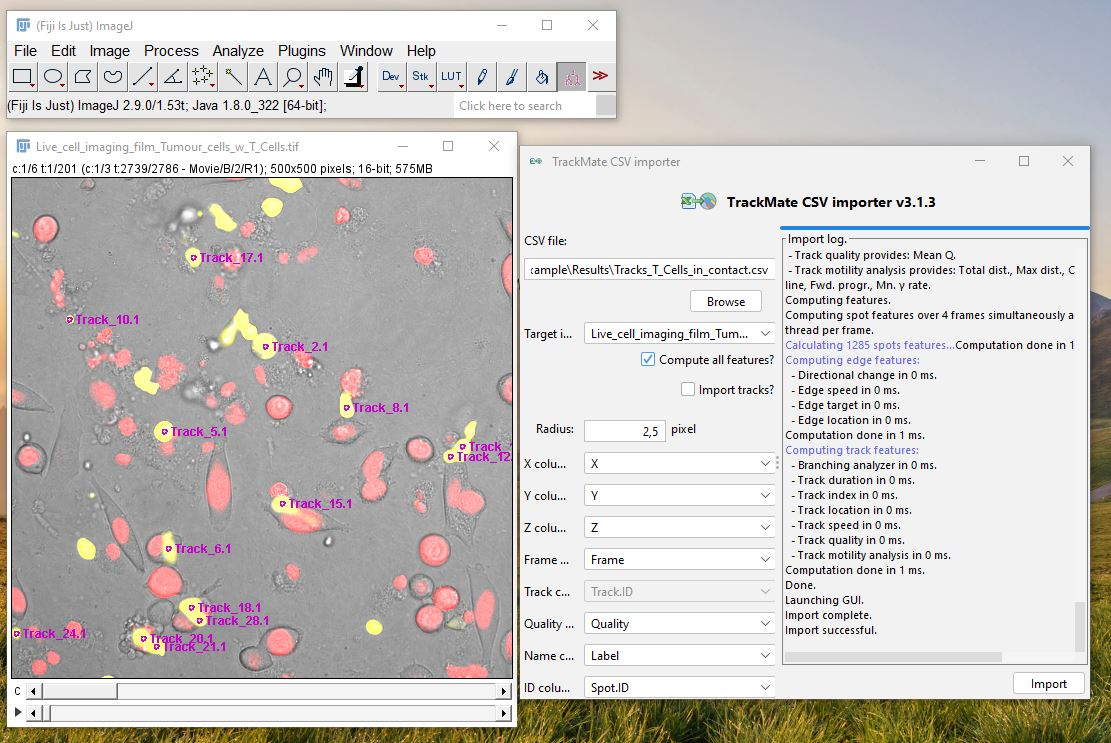
\includegraphics[width=0.9\textwidth]{Screenshot_TrackMate_CSV_Importer.JPG}
\caption[TrackMate_CSV_Importer]{Via the TrackMate CSV Importer GUI, we can load our computed cell-cell contacts back into a TrackMate session. \label{TrackMate_CSV_Importer}}
\end{figure}

\paragraph{Correlating results to immunological staining results}
We often want to connect the dynamic information of the cell tracks to the static information of the same cells from immunological staining. For this, we provide the function \codeword{match_to_endpoint_ROIs()} to match the cell tracks to the corresponding cell ROIs at the end point. The function \codeword{add_meas_to_matches()} can add the measurements of the signal intensity to the mapping of cell tracks to endpoint ROIs (\textcolor{darkblue}{add a schematic figure?}).

%\paragraph{Identifying dying tumour cells}
%\textcolor{blue}{[...]}

\paragraph{Computing characteristics of cell tracks} To get a thorough picture of the mechanisms behind T cell killing, we observe additional aspects of T cell dynamics including speed, directionality and persistence of the cells. To compute and to cluster these cell track characteristics, we use the package \textit{celltrackR} by Ingel Wortel et al \citep{RN299}. The documentation of this package can be found at \url{https://ingewortel.github.io/celltrackR/}.

\paragraph{Exporting and visualization of results}
To check of the computed cell-cell contacts, we export the track information of the T cells that were in contact as .csv-file using \codeword{prepareExportContacts()} and \codeword{write.csv()}. The exported files are loaded into TrackMate via ImageJ > Plugins > Tracking > TrackMate CSV Importer. Using the .csv file, TrackMate labels the T cells in the .tif-file only during a contact (see Figure \ref{TrackMate_CSV_Importer}). This allows us to revisit the live-cell imaging film and to check whether cell-cell contacts are correctly computed.

%===================================================
\section{Quality control}

\paragraph{Segmentation and track quality}  To identify cell-cell contacts, correct segmentation and tracking data are pivotal. Already during the analysis with TrackMate, we filter the segmented cells and their corresponding tracks by the spot size, the mean fluorescence intensity, the track length and other criteria \citep{RN293}. After importing the data into R, we detect and correct for artefacts, e.g.,  double tracking or drift, via track angle analyses from the package \textit{celltrackR} by Ingel Wortel et al \citep{RN299}. 

\paragraph{Evaluation metric}
To assess the reliability of cell contact detection, we manually observe cell-cell contacts in the films and afterwards, we evaluate the accordance of the computed cell-cell contacts to the manually obtained results.
In addition, we import the detected cell-cell contacts back into TrackMate such that cells are labelled in the film during a cell-cell contact.

%%===================================================
\chapter{Results}


\section{Accuracy of cell segmentation and cell tracking}

Discuss
\begin{itemize}
	\item Accuracy of StarDist (especially on mitotic cells and T cells in a non-regular shape)
	\item Accuracy of LAP tracker (include photos)?
\end{itemize}

\section{Accuracy of cell-cell contact detection}

\begin{itemize}
	\item Detection based on duration of proximity (not consideration of cell shape)
	\item Allows simultaneous contact of one T cell to multiple tumour cells?
	\item Figure: Boxplot to demonstrate deviation from ground truth?
\end{itemize}

\section{Evaluating computation time}

\begin{itemize}
	\item Compute complexity for the approach with and without grid
	\item Include benchmarking results
\end{itemize}

\section{Detecting tumour cell/T cell contacts}

\begin{itemize}
	\item Olis Data with ground truth
	\item Olis Data on large scale
	\item Olis Data - Compare with and without OVA
	\item Olis Data - Connect to Fix-While-Filming
	\item Steffens Data with ground truth
	\item Steffens Data on large scale
\end{itemize}

%===================================================
\chapter{Discussion}
%===================================================

\section{Reliability and potential}

\begin{itemize}
	\item Discuss results (comparison to ground truth)
\end{itemize}

\section{Compared methods}

\begin{itemize}
	\item Imaris
	\item CellProfiler
	\item Napari
\end{itemize}

\section{Biological interpretation and perspective}

\begin{itemize}
	\item Interpretation of results
	\item Perspective of potential experiments/analyses
\end{itemize}

%===================================================
\chapter{Conclusion}
%===================================================

In this thesis, we set up a framework for an automatic detection of cell-cell contacts in live-cell imaging films. This enables a quantitative analysis of dynamic cell data.
The framework relies on previous segmentation and tracking of cells using well-established open-source tools. If the segmentation and tracking is accurate, the cell-cell contact detection based on the duration of cell proximity proved to be

\begin{itemize}
	\item Created a framework
	\item R package automatizes cell-cell contact detection -> comparability (observer bias avoided)
\end{itemize}


%%===================================================
\chapter*{Supplement}

\begin{itemize}
	\item Link to R package on GitHub
	\item Link to movies?
\end{itemize}
%%===================================================


%%===================================================
%\chapter*{Acknowledgment}
%\addcontentsline{toc}{chapter}{Acknowledgment}



%===================================================
%
%\listoffigures
%\listoftables
%===================================================
\bibliographystyle{unsrtnat}
\renewcommand{\bibname}{References}
\bibliography{literatur}


%%===================================================
%\chapter*{Supplement}
%\addcontentsline{toc}{chapter}{Supplementary}
%
%\newcommand{\beginsupplement}{
%        \setcounter{table}{0}
%        \renewcommand{\thetable}{S\arabic{table}}%
%        \setcounter{figure}{0}
%        \renewcommand{\thefigure}{S\arabic{figure}}%
%     }
% 
%\beginsupplement



\end{document}